\documentclass{standalone}
\usepackage{tikz}
\usepackage{amsmath}
\usepackage{xcolor}
\usetikzlibrary{arrows.meta, decorations.pathreplacing, backgrounds, positioning, calc}

% Define custom colors
\definecolor{softyellow}{HTML}{F2D648}
\definecolor{dustyblue}{HTML}{9EB9D4}
\definecolor{berkeleyblue}{RGB}{0, 50, 98}
\definecolor{berkeleygold}{RGB}{253, 181, 21}

\begin{document}

\begin{minipage}{0.33\textwidth}
\begin{center}
    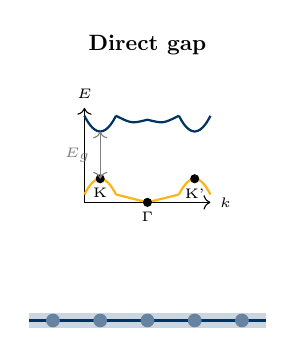
\begin{tikzpicture}[scale=1]
      \begin{scope}[shift={(0,1.5)}]
        \draw[->] (-0.8,0) -- (0.8,0) node[right] {\tiny \textcolor{black}{$k$}};
        \draw[->] (-0.8,0) -- (-0.8,1.2) node[above] {\tiny \textcolor{black}{$E$}};
        \draw[berkeleyblue, thick] (-0.8,1.1) parabola bend (-0.6,0.9) (-0.4,1.1);
        \draw[berkeleyblue, thick] (-0.4,1.1) .. controls (-0.2,1.0) .. (0,1.05)
                                   .. controls (0.2,1.0) .. (0.4,1.1);
        \draw[berkeleyblue, thick] (0.4,1.1) parabola bend (0.6,0.9) (0.8,1.1);
        \draw[berkeleygold, thick] (-0.8,0.1) parabola bend (-0.6,0.3) (-0.4,0.1);
        \draw[berkeleygold, thick] (-0.4,0.1) .. controls (-0.2,0.05) .. (0,0)
                                  .. controls (0.2,0.05) .. (0.4,0.1);
        \draw[berkeleygold, thick] (0.4,0.1) parabola bend (0.6,0.3) (0.8,0.1);
        \filldraw[black] (-0.6,0.3) circle (0.05) node[below] {\tiny K};
        \filldraw[black] (0.6,0.3) circle (0.05) node[below] {\tiny K'};
        \filldraw[black] (0,0) circle (0.05) node[below] {\tiny $\Gamma$};
        \draw[<->, gray] (-0.6,0.3) -- (-0.6,0.9) node[midway, left] {\tiny $E_g$};
        \node[scale=0.8] at (0,2) {\textbf{Direct gap}};
      \end{scope}

      \fill[berkeleyblue!20] (-1.5,-0.1) rectangle (1.5,0.1);
      \draw[very thick, berkeleyblue] (-1.5,0) -- (1.5,0);
      \foreach \x in {-1.2,-0.6,0,0.6,1.2} {
        \filldraw[berkeleyblue!60] (\x,0) circle (0.08);
      }
    \end{tikzpicture}
\end{center}
\end{minipage}%
%
\begin{minipage}{0.33\textwidth}
\begin{center}
    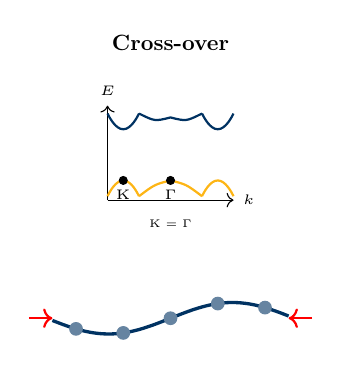
\begin{tikzpicture}[scale=1]
      \begin{scope}[shift={(0,1.5)}]
        \draw[->] (-0.8,0) -- (0.8,0) node[right] {\tiny \textcolor{black}{$k$}};
        \draw[->] (-0.8,0) -- (-0.8,1.2) node[above] {\tiny \textcolor{black}{$E$}};
        \draw[berkeleyblue, thick] (-0.8,1.1) parabola bend (-0.6,0.9) (-0.4,1.1);
        \draw[berkeleyblue, thick] (-0.4,1.1) .. controls (-0.2,1.0) .. (0,1.05)
                                   .. controls (0.2,1.0) .. (0.4,1.1);
        \draw[berkeleyblue, thick] (0.4,1.1) parabola bend (0.6,0.9) (0.8,1.1);
        \draw[berkeleygold, thick] (-0.8,0.05) parabola bend (-0.6,0.25) (-0.4,0.05);
        \draw[berkeleygold, thick] (-0.4,0.05) .. controls (-0.2,0.2) .. (0,0.25)
                                  .. controls (0.2,0.2) .. (0.4,0.05);
        \draw[berkeleygold, thick] (0.4,0.05) parabola bend (0.6,0.25) (0.8,0.05);
        \filldraw[black] (-0.6,0.25) circle (0.05) node[below] {\tiny K};
        \filldraw[black] (0,0.25) circle (0.05) node[below] {\tiny $\Gamma$};
        \node[scale=0.8] at (0,-0.3) {\tiny K = $\Gamma$};
        \node[scale=0.8] at (0,2) {\textbf{Cross-over}};
      \end{scope}

      \draw[very thick, berkeleyblue] plot[smooth, domain=-1.5:1.5] (\x, {0.2*sin(2*\x*180/pi)});
      \foreach \x in {-1.2,-0.6,0,0.6,1.2} {
        \filldraw[berkeleyblue!60] (\x,{0.2*sin(2*\x*180/pi)}) circle (0.08);
      }
      \draw[thick, red, ->] (-1.8,0) -- (-1.5,0);
      \draw[thick, red, ->] (1.8,0) -- (1.5,0);
    \end{tikzpicture}
\end{center}
\end{minipage}%
%
\begin{minipage}{0.33\textwidth}
\begin{center}
    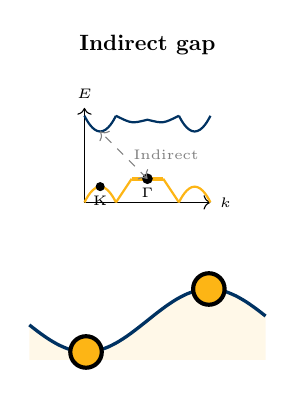
\begin{tikzpicture}[scale=1]
      \begin{scope}[shift={(0,1.5)}]
        \draw[->] (-0.8,0) -- (0.8,0) node[right] {\tiny \textcolor{black}{$k$}};
        \draw[->] (-0.8,0) -- (-0.8,1.2) node[above] {\tiny \textcolor{black}{$E$}};
        \draw[berkeleyblue, thick] (-0.8,1.1) parabola bend (-0.6,0.9) (-0.4,1.1);
        \draw[berkeleyblue, thick] (-0.4,1.1) .. controls (-0.2,1.0) .. (0,1.05)
                                   .. controls (0.2,1.0) .. (0.4,1.1);
        \draw[berkeleyblue, thick] (0.4,1.1) parabola bend (0.6,0.9) (0.8,1.1);
        \draw[berkeleygold, thick] (-0.8,0) parabola bend (-0.6,0.2) (-0.4,0);
        \draw[berkeleygold, thick] (-0.4,0) .. controls (-0.3,0.15) .. (-0.2,0.3);
        \draw[berkeleygold, ultra thick] (-0.2,0.3) -- (0.2,0.3);
        \draw[berkeleygold, thick] (0.2,0.3) .. controls (0.3,0.15) .. (0.4,0);
        \draw[berkeleygold, thick] (0.4,0) parabola bend (0.6,0.2) (0.8,0);
        \filldraw[black] (0,0.3) circle (0.06) node[below] {\tiny $\Gamma$};
        \filldraw[black] (-0.6,0.2) circle (0.05) node[below] {\tiny K};
        \draw[<->, gray, dashed] (0,0.3) -- (-0.6,0.9) node[midway, right] {\tiny Indirect};
        \node[scale=0.8] at (0,2) {\textbf{Indirect gap}};
      \end{scope}

      \fill[berkeleygold!10] plot[smooth, domain=-1.5:1.5] (\x, {0.4*sin(2*\x*180/pi)})
        -- (1.5,-0.5) -- (-1.5,-0.5) -- cycle;
      \draw[very thick, berkeleyblue] plot[smooth, domain=-1.5:1.5] (\x, {0.4*sin(2*\x*180/pi)});
      \foreach \x in {-0.78,0.78} {
        \filldraw[fill=berkeleygold, draw=black, line width=1.5pt] 
          (\x,{0.4*sin(2*\x*180/pi)}) circle (0.2);
      }
    \end{tikzpicture}
\end{center}
\end{minipage}



\end{document}
